\documentclass[10pt,twoside]{article}
\usepackage[utf8]{inputenc}
\usepackage{amsmath}
\usepackage{amsfonts}
\usepackage{amssymb}
\usepackage[spanish,es-noshorthands]{babel}
\usepackage[T1]{fontenc}
\usepackage{lmodern}
\usepackage{graphicx,hyperref}
\usepackage{tikz,pgf}
\usepackage{multicol}
\usepackage{subfig}
\usepackage[papersize={6.5in,8.5in},width=5.5in,height=7in]{geometry}
%\usepackage{fancyhdr}
%\pagestyle{fancy}
%\fancyhead[LE]{
\includegraphics[height=12pt]{Images/logo-colegio.png} %Asig $^{\circ}$}
%\fancyhead[RE]{}
%\fancyhead[RO]{\textit{Germ\'an Avenda\~no Ram\'irez, Lic. U.D., M.Sc. U.N.}}
%\fancyhead[LO]{}

\author{Germ\'an Avenda\~no Ram\'irez \thanks{Lic. U.D., M.Sc. U.N., \underline{Email:} matematicas.german@gmail.com}}
\title{\begin{minipage}{.2\textwidth}

\includegraphics[height=1.75cm]{Images/logo-colegio.png}\end{minipage}
\begin{minipage}{.55\textwidth}
\begin{center}
Taller 01\\
Principios morales\\
\'{E}tica $9^{\circ}$
\end{center}
\end{minipage}\hfill
\begin{minipage}{.2\textwidth}

\includegraphics[height=1.75cm]{Images/logo-sed.png} 
\end{minipage}}
\date{}
\begin{document}
\maketitle
Nombre: \hrulefill Curso: \underline{\hspace*{44pt}} Fecha: \underline{\hspace*{2.5cm}}
\subsection{Aprendo algo nuevo}
\subsubsection*{Principios morales}
Son normas o reglas de conducta de carácter general o \emph{universal}, que orientan la acción del ser humano como ser social. Son principios en la medida en que se constituyen como base, \emph{fundamento} o cimiento de la actividad humana, para que esta garantice la supervivencia y el buen desarrollo de las comunidades y de los individuos.

En este sentido, los principios morales son el producto de la definición o la determinación de acciones y cosas que los seres humanos han señalado como inapropiados o inaceptables en determinadas circunstancias o en determinada época de la historia, creando leyes, máximas o preceptos para contrarrestarlos. De esta forma se determina como bueno o malo, correcto o incorrecto, apropiado o inapropiado, obligatorio o permitido, cualquier acción o decisión que tenga relación con la supervivencia y el bienestar de la especie, organizada en comunidades, y se crean mecanismos y medidas para evitar los efectos adversos.

En ocasiones dichas determinaciones y sus correspondientes leyes y preceptos, favorecieron a algunos individuos o comunidades, en detrimento de otras personas y grupos.

Por ejemplo, cuando la esclavitud fue aceptada moralmente por algunas sociedades o las mujeres fueron consideradas inferiores a los hombres. De forma afortunada y progresiva la humanidad se ha acercado a la comprensión y aceptación de la igualdad de todos los seres humanos, sin consideraciones de raza, sexo, credo o cualquier otra condición. En consecuencia, los principios morales se van haciendo realmente universales, sobrepasando los límites de las comunidades y de las naciones hasta llegar a relacionarse con el respeto a la vida, el amor al prójimo, la atención a los s, el cuidado del medio ambiente, la solidaridad, la integridad y la responsabilidad, entre muchos otros comportamientos de respeto y actitud práctica y razonable, con el mismo objetivo de preservar la especie humana y garantizar su desarrollo armónico.
\subsection{Ejercito lo aprendido}
Responda las preguntas en su cuaderno. Contraste las respuestas con un compañero o compañera.
\begin{enumerate}
\item ¿Cuáles pueden ser algunos principios morales relacionados con la integridad?
\item Mencione por lo menos cinco acciones que considere principios morales que contribuyan a la supervivencia de la especie
\item ¿De qué manera la verdad, la honradez y la puntualidad, pueden considerarse principios morales?
\end{enumerate}
\subsection{Aprendo algo nuevo}
\subsection*{Juicio vs norma}
El \emph{juicio} puede ser definido como el análisis y valoración de un asunto, donde se afirma o niega algo, se distingue lo positivo o negativo del mismo, o se establece lo correcto o incorrecto de un hecho, a la luz de una determinada
normatividad.

Una \emph{norma} por su parte, es una regla o conjunto de reglas con criterio de valor que pretenden establecer un orden de comportamiento, para regular la participación y conducta del individuo en la sociedad. Estas se han establecido para prohibir, obligar, permitir o prevenir determinados actos o comportamientos.

Las normas obran como el timón que sirve para mantener a la sociedad en el rumbo que ella misma ha determinado, por ello son de valor funcional considerable pues organizan y cohesionan a los individuos en torno a unas costumbres y conductas que mantienen la organización del grupo y preservan la estabilidad social, dentro de la ruta que ha de llevarla a sus objetivos.

Como se afirmó en el tema anterior, cada sociedad determina sus propias normas, en su momento histórico, acorde a sus intereses y circunstancias. Los espartanos, por ejemplo, establecieron sus normas como sociedad guerrera; el feudalismo determinó sus normas sobre bases de desigualdad social, de inequidad y despotismo, arguyendo que el poder y los privilegios venían directamente de Dios. Unos y otros, establecían sus juicios de acuerdo a esos marcos sociales, a sus costumbres, a su normatividad.

Aquí podemos deducir que el juicio ético social está basado en
la norma social, responde a ella y a la sociedad que la estableció, pero no está necesariamente en armonía con criterios de justicia y universalidad. Entre más estrechos son los límites e intereses de una sociedad, menos universales serán sus normas y menos justos serán sus juicios. La universalidad de las normas acercan los derechos para todos
los individuos, reparten cargas y deberes de manera, garantizan para todos la participación igual del progreso y del desarrollo, convierte a la sociedad en una comunidad respetuosa e incluyente, con futuro para sí y para sus miembros.
\subsection{Ejercito lo aprendido}
\begin{enumerate}
\item En parejas, cada uno se har\'{a} cargo de unas dos o tres áreas específicas del contexto (familia, barrio, \ldots) y elaborará un conjunto de normas que garanticen, en su criterio, un mejor bienestar para cada \'{a}rea.
\item Expongan su trabajo en el curso y sometan a discusi\'{o}n la validez de la normatividad redactada.
\end{enumerate}
\section*{Constituci\'{o}n pol\'{i}tica y organizaci\'{o}n del estado}
\subsection{Lo que s\'{e}}
Antes de comenzar, observe las fotograf\'{i}as y responda en su cuaderno:
\begin{center}
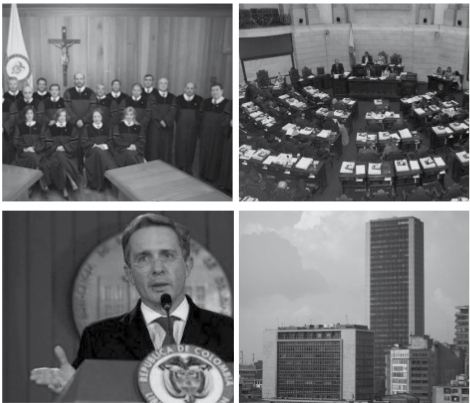
\includegraphics[scale=.75]{Images/congreso.png} 
\end{center}
\begin{enumerate}
\item ¿Cu\'{a}les son las funciones del congreso? ¿Quienes son sus miembros?
\item ¿Qu\'{e} requisitos son necesarios para ser elegido Presidente de Colombia?
\item ¿Cu\'{a}les son los organismos encargados de impartir justicia en Colombia?
\item ¿En qu\'{e} situaciones intervienen la Contralor\'{i}a, la Procurador\'{i}a y la Defensor\'{i}a del Pueblo?
\item ¿Cu\'{a}les son los organismos encargados de dirigir los asuntos en tu municipio?
\end{enumerate}
\subsection{Aprendo algo nuevo}
\subsubsection*{Estructura de la constituci\'{o}n}
La Constitución Política es el máximo documento legal de un Estado democrático y soberano. Todas las leyes, decretos y normas deben estar en armonía con el espíritu de la Constitución y las determinaciones allí dispuestas. Para facilitar su conocimiento y consulta, el documento escrito tiene la siguiente estructura:
\begin{center}
\begin{tikzpicture}
\node[rectangle,draw] {Títulos}
[level distance=15mm]
child {node[rectangle,draw] {Cap\'{i}tulos}
child {node[rectangle,draw] {Art\'{i}culos}}
};
\end{tikzpicture}
\end{center}
\end{document}
